\section{Extract-Transform-Load (ETL) Script}
\label{sec:etl_script}

The ETL pipeline takes the raw 2025 file from its source, converts it into the tables of the warehouse, and loads them into PostgreSQL 17. It is implemented in Python using Apache Airflow.

\subsection{Design Constraints}
\label{subsec:etl_constraints}

The following constraints are considered in the implementation of the ETL pipeline:
\begin{enumerate}
    \item Because the uncompressed CSV file is 3.37\,GB and risks exhausting available RAM under full ingestion, we delegate all parsing and transformation to DuckDB \cite{raasveldt2019duckdb}. DuckDB processes the input out-of-core in a streaming pipeline, constrained to a 2\,GB memory limit and 4 execution threads.
    \item Row-by-row \sql{INSERT} statements are slow at this volume. Each inserted row updates every index on the table and is checked against every foreign key. The PostgreSQL documentation recommends loading large tables with \sql{COPY}, creating indexes after the data is in, and dropping foreign key constraints during the load \cite{postgresql2025populating}.
\end{enumerate}

\subsection{Pipeline Architecture}
\label{subsec:etl_architecture}

\begin{figure}[t]
\centering
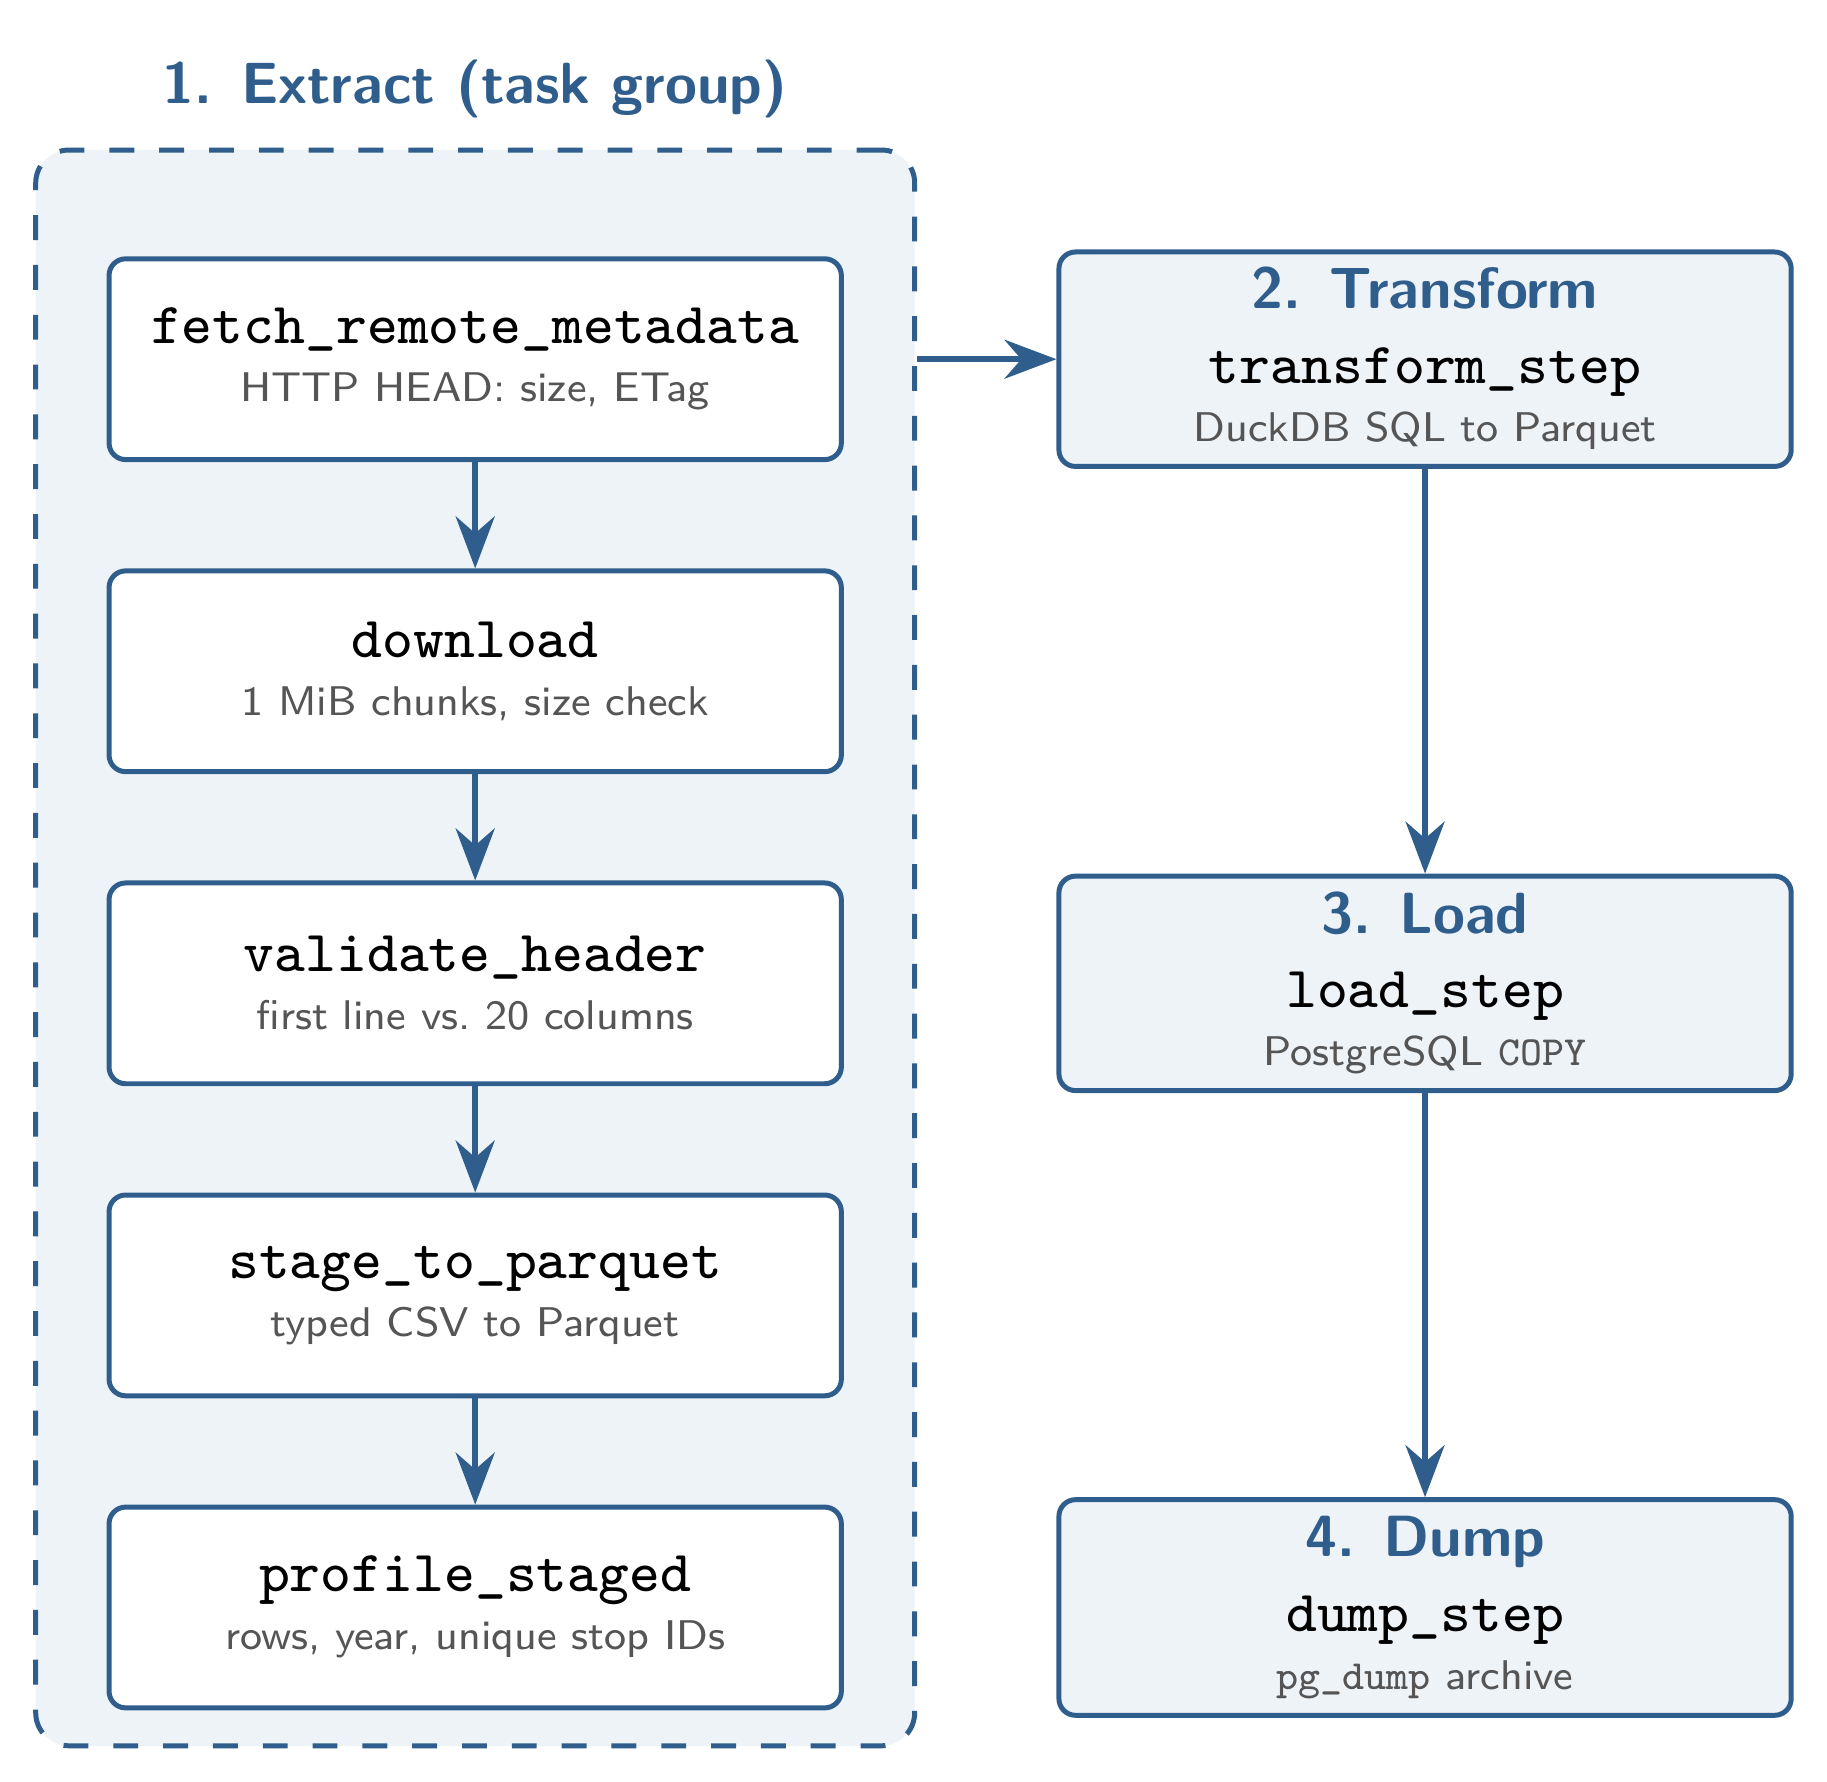
\includegraphics[width=\columnwidth]{figures/etl_dag.png}
\caption{Tasks of the \texttt{dutch\_railway\_etl} Airflow DAG.}
\Description{The Airflow DAG runs an extract task group of five tasks, then a transform task, a load task, and a dump task, in sequence.}
\label{fig:etl_dag_flow}
\end{figure}

The DAG \texttt{dutch\_railway\_etl} runs four stages in sequence (Figure~\ref{fig:etl_dag_flow}). Each task retries twice before failing. Every file the pipeline writes is first written under a temporary \texttt{.part} name and then renamed, so a failed task never leaves a half-written file in place of a complete one.

\subsubsection{Extract}
\label{subsubsec:extraction}

\texttt{fetch\_remote\_metadata} sends an HTTP \texttt{HEAD} request to the source and reads the file size and \texttt{ETag}. \texttt{download} skips the download when a local copy exists whose size and \texttt{ETag} match the values saved in a sidecar file from the previous run. Otherwise it streams the file to disk in 1\,MiB chunks and checks the number of bytes received against the reported size before renaming the file. \texttt{validate\_header} reads only the first line of the compressed file and checks that the column names and their order match the expected 20 columns.

\texttt{stage\_to\_parquet} then has DuckDB read the CSV with an explicit type for every column instead of letting it guess types, and writes it to a Zstandard-compressed Parquet file. The session time zone is set to \texttt{Europe/Amsterdam} so that all timestamps are read in Dutch local time. Finally, \texttt{profile\_staged} checks that the staged file is not empty, that every service date falls in the requested year, and that \texttt{Stop:RDT-ID} is unique.

\subsubsection{Transform}
\label{subsubsec:transformation}

The transform stage defines a DuckDB view over the staged file and runs one SQL query per warehouse table. The view applies the station code corrections and adds a sort key for the stops of a service, ordered by time and then by stop identifier. Each query writes its result to its own Parquet file. \texttt{dim\_date} is generated with one row per day between the first and the last service date. \texttt{dim\_time} is generated with one row for each of the 1,440 minutes of a day. \texttt{dim\_station}, \texttt{fact\_service}, and \texttt{fact\_stop} are derived from the staged rows. Table~\ref{tab:transformation_rules} lists the rules applied to individual columns.

\begin{table*}[t]
\centering
\small
\caption{Transformation rules}
\Description{Rules applied to individual warehouse columns during the transform stage, with the reason for each.}
\label{tab:transformation_rules}
\begin{tabular}{>{\raggedright\arraybackslash}p{0.27\textwidth} >{\raggedright\arraybackslash}p{0.68\textwidth}}
\toprule
\textbf{Column} & \textbf{Rule} \\
\midrule
\texttt{dim\_station.station\_code} &
\texttt{LAND} with the name Venezia Santa Lucia becomes \texttt{VENEZ}, and \texttt{BERHBT} becomes \texttt{BERHBL}. Each code then names exactly one station, and Berlin Hbf has one code. \\
\addlinespace
\texttt{dim\_date.date\_key} &
The date as an integer of the form YYYYMMDD, for example 20250312. A year can be selected with a range on the key without joining \texttt{dim\_date}. \\
\addlinespace
\texttt{dim\_time.time\_key}, \texttt{fact\_stop.arrival\_time}, \texttt{fact\_stop.departure\_time} &
The time as an integer of the form HHMM, for example 1430 for 14:30. Seconds are dropped, which affects the 4,961 stops whose times are not on a whole minute. \\
\addlinespace
\texttt{dim\_time.time\_of\_day} &
\texttt{morning} from 05:00 to 11:59, \texttt{afternoon} from 12:00 to 17:59, and \texttt{night} from 18:00 to 04:59. \\
\addlinespace
\texttt{fact\_service.cancel\_status} &
\texttt{completely} if the completely cancelled flag is set, otherwise \texttt{partially} if the partly cancelled flag is set, otherwise \texttt{none}. The completely cancelled flag is checked first because it is usually set together with the other one. \\
\addlinespace
\texttt{fact\_service.first\_train\_number}, \texttt{last\_train\_number}, \texttt{train\_id\_changed} &
The train number at the first and at the last stop of the service, and whether the service has more than one train number. \\
\addlinespace
\texttt{fact\_stop.cancel\_status} &
\texttt{completely} if both the arrival and the departure are cancelled, \texttt{arrival-only} or \texttt{departure-only} if one of them is, and \texttt{none} otherwise. A missing arrival at the origin or a missing departure at the terminus counts as cancelled, so a cancelled origin or terminus is \texttt{completely} cancelled. \\
\addlinespace
\texttt{fact\_stop.arrival\_delay}, \texttt{fact\_stop.departure\_delay} &
\sql{NULL} when the arrival or departure is cancelled, and the source delay otherwise. Averages then only include stops that were served. \\
\addlinespace
\texttt{fact\_stop.arrival\_day\_offset}, \texttt{fact\_stop.departure\_day\_offset} &
The number of days between the service date and the arrival or departure, so that stops after midnight keep their correct order. \\
\bottomrule
\end{tabular}
\end{table*}


After writing the tables, the transform stage checks them before anything is loaded. It verifies that \texttt{fact\_stop} has as many rows as the staged file, that no station code has more than one name, and that every foreign key value in the fact tables exists in the table it refers to.

\subsubsection{Load}
\label{subsubsec:loading}

The load stage puts the transformed tables into the PostgreSQL warehouse. It runs as a single transaction, so a run that fails leaves no partly loaded tables behind.

The loader creates the warehouse tables from \texttt{schema.sql}, including their indexes and foreign keys, and copies the rows of each table into PostgreSQL with \sql{COPY}. The dimensions are loaded first, then \texttt{fact\_service}, then \texttt{fact\_stop}.

To make the copy of 22 million stops faster, the loader removes the indexes and foreign keys of the fact tables before the copy and restores them afterwards. PostgreSQL then builds each index and checks each foreign key once over the whole table instead of once per row, as the PostgreSQL documentation recommends for bulk loads \cite{postgresql2025populating}. The finished tables have all the indexes and constraints defined in \texttt{schema.sql}.

\subsubsection{Dump}
\label{subsubsec:dump}

The last stage writes the five warehouse tables to a \texttt{pg\_dump} archive in custom format.

\subsection{Schema Constraints}
\label{subsec:schema_constraints}

The warehouse enforces the following constraints.
\begin{itemize}
    \item \textbf{Primary keys} on \texttt{date\_key}, \texttt{time\_key}, \texttt{station\_code}, \texttt{rdt\_id}, and \texttt{stop\_id}.
    \item \textbf{Foreign keys} from \texttt{fact\_service} to \texttt{dim\_date}, and from \texttt{fact\_stop} to \texttt{fact\_service}, \texttt{dim\_station}, and \texttt{dim\_time}. \texttt{fact\_stop} refers to \texttt{dim\_time} twice, once for the arrival and once for the departure. Both of these columns allow \sql{NULL} for the origin and the terminus.
    \item \textbf{Check constraints} that limit \texttt{time\_of\_day} and the two \texttt{cancel\_status} columns to the values listed in Table~\ref{tab:transformation_rules}.
    \item \textbf{Secondary indexes} on the foreign key columns used in joins, which are \texttt{fact\_service(date\_key)}, \texttt{fact\_stop(rdt\_id)}, and \texttt{fact\_stop(station\_code)}.
\end{itemize}

\subsection{Issues and Solutions}
\label{subsec:etl_issues}

Table~\ref{tab:etl_issues} lists the problems we had to handle while building the pipeline and how each one was solved.

\begin{table*}[t]
\centering
\small
\caption{Issues handled by the ETL pipeline}
\Description{Summary of data engineering challenges, symptoms, and mitigations implemented in the ETL pipeline.}
\label{tab:etl_issues}
\begin{tabularx}{\textwidth}{l X X}
\toprule
\textbf{Issue} & \textbf{Problem} & \textbf{Solution} \\
\midrule
\textbf{Load speed} &
Inserting 22.2 million rows into tables with indexes and foreign keys updates every index and checks every key for each row. &
Drop the fact table foreign keys and secondary indexes, load with \sql{COPY}, and rebuild them once after the load \cite{postgresql2025populating}. \\
\addlinespace

\textbf{Memory} &
The decompressed file is 3.37\,GB, too large to read into Python memory. &
Read and transform the file in DuckDB with a 2\,GB memory limit, and keep only Parquet files between stages \cite{raasveldt2019duckdb}. \\
\addlinespace

\textbf{Incomplete downloads} &
A dropped connection can leave a truncated file that looks like a valid download. &
Download to a \texttt{.part} file, compare its size with \texttt{Content-Length}, and rename it only if the sizes match. \\
\addlinespace

\textbf{Station codes} &
\texttt{LAND} has two station names, and Berlin Hbf has two codes. &
Remap Venezia Santa Lucia to \texttt{VENEZ} and merge \texttt{BERHBT} into \texttt{BERHBL} during the transform. \\
\addlinespace

\textbf{Delays of cancelled stops} &
About 1.1 million cancelled arrivals and departures have a delay of 0, which would count them as on time. &
Store these delays as \sql{NULL}. \\
\addlinespace

\textbf{Stops after midnight} &
Stops after midnight would get the date of their service, which is the previous day. &
Store an arrival and a departure day offset relative to the service date in \texttt{fact\_stop}. \\
\bottomrule
\end{tabularx}
\end{table*}
